%%%%%%%%%%%%%%%%%%%%%%%%%%%%%%%%%%%%%%%%%%%%%%%%%%%%%%%%%%%%%%%%%%%%%%%%%%%%%%%
% LaTeX Document Template
%
% Author: Léonard Bise
% Date: 09.07.2018
%
%%%%%%%%%%%%%%%%%%%%%%%%%%%%%%%%%%%%%%%%%%%%%%%%%%%%%%%%%%%%%%%%%%%%%%%%%%%%%%%

% Settings of the template
%%%%%%%%%%%%%%%%%%%%%%%%%%%%%%%%%%%%%%%%%%%%%%%%%%%%%%%%%%%%%%%%%%%%%%%%%%%%%%%
% Template Settings
%
% Author: Léonard Bise
% Date: 25.05.2018
%
%%%%%%%%%%%%%%%%%%%%%%%%%%%%%%%%%%%%%%%%%%%%%%%%%%%%%%%%%%%%%%%%%%%%%%%%%%%%%%%

%\documentclass[11pt,a4paper, openany]{memoir}
\documentclass[a4paper,11pt,fleqn]{book}

\usepackage[utf8]{inputenc}
\usepackage[T1]{fontenc}
\usepackage[french]{babel}

\usepackage{booktabs}
\usepackage{longtable}
\usepackage[paper=portrait,pagesize]{typearea}

\usepackage{fourier} % Utopia font-typesetting including mathematical formula compatible with newer TeX-Distributions (>2010)
%\usepackage{utopia} % on older systems -> use this package instead of fourier in combination with mathdesign for better looking results
%\usepackage[adobe-utopia]{mathdesign}
\setlength{\textwidth}{146.8mm} % = 210mm - 37mm - 26.2mm
\setlength{\oddsidemargin}{11.6mm} % 37mm - 1in (from hoffset)
\setlength{\evensidemargin}{0.8mm} % = 26.2mm - 1in (from hoffset)
\setlength{\topmargin}{-2.2mm} % = 0mm -1in + 23.2mm 
\setlength{\textheight}{221.9mm} % = 297mm -29.5mm -31.6mm - 14mm (12 to accomodate footline with pagenumber)
\setlength{\headheight}{14pt}

\usepackage{setspace} % increase interline spacing slightly
\setstretch{1.1}

\makeatletter
\setlength{\@fptop}{0pt}  % for aligning all floating figures/tables etc... to the top margin
\makeatother

\usepackage[explicit]{titlesec}
%\titlespacing*{\chapter}{0pt}{5pt}{*0}
\titlespacing*{\chapter}{0pt}{3.5ex plus 1ex minus .2ex}{2.3ex plus .2ex}
\titlespacing*{\section}{0pt}{3.5ex plus 1ex minus .2ex}{2.3ex plus .2ex}
\titlespacing*{\subsection}{0pt}{3.5ex plus 1ex minus .2ex}{2.3ex plus .2ex}
\titlespacing*{\subsubsection}{0pt}{3.5ex plus 1ex minus .2ex}{2.3ex plus .2ex}
%\titlespacing*{\section}{0pt}{13.2pt}{*0}  % 13.2pt is line spacing for a text with 11pt font size
%\titlespacing*{\subsection}{0pt}{13.2pt}{*0}
%\titlespacing*{\subsubsection}{0pt}{13.2pt}{*0}

\newcommand*\chapterlabel{}
%\renewcommand{\thechapter}{\Roman{chapter}}
\titleformat{\chapter}[display]  % type (section,chapter,etc...) to vary,  shape (eg display-type)
	{\normalfont\bfseries\Huge} % format of the chapter
	{\gdef\chapterlabel{\thechapter\ }}     % the label 
 	{0pt} % separation between label and chapter-title
 	  {\begin{tikzpicture}[remember picture,overlay]
    \node[yshift=-8cm] at (current page.north west)
      {\begin{tikzpicture}[remember picture, overlay]
        \draw[fill=black] (0,0) rectangle(35.5mm,15mm);
        \node[anchor=north east,yshift=-7.2cm,xshift=34mm,minimum height=30mm,inner sep=0mm] at (current page.north west)
        {\parbox[top][30mm][t]{15mm}{\raggedleft $\phantom{\textrm{l}}$\color{white}\chapterlabel}};  %the black l is just to get better base-line alingement
        \node[anchor=north west,yshift=-7.2cm,xshift=37mm,text width=\textwidth,minimum height=30mm,inner sep=0mm] at (current page.north west)
              {\parbox[top][30mm][t]{\textwidth}{\color{black}#1}};
       \end{tikzpicture}
      };
   \end{tikzpicture}
   \gdef\chapterlabel{}
  } % code before the title body

\newcounter{myparts}
\newcommand*\partlabel{}
\titleformat{\part}[display]  % type (section,chapter,etc...) to vary,  shape (eg display-type)
	{\normalfont\bfseries\Huge} % format of the part
	{\gdef\partlabel{\thepart\ }}     % the label 
 	{0pt} % separation between label and part-title
 	  {\setlength{\unitlength}{20mm}
	  \addtocounter{myparts}{1}
	  \begin{tikzpicture}[remember picture,overlay]
    \node[anchor=north west,xshift=-65mm,yshift=-6.9cm-\value{myparts}*20mm] at (current page.north east) % for unknown reasons: 3mm missing -> 65 instead of 62
      {\begin{tikzpicture}[remember picture, overlay]
        \draw[fill=black] (0,0) rectangle(62mm,20mm);   % -\value{myparts}\unitlength
        \node[anchor=north west,yshift=-6.1cm-\value{myparts}*20mm,xshift=-60.5mm,minimum height=30mm,inner sep=0mm] at (current page.north east)
        {\parbox[top][30mm][t]{55mm}{\raggedright \color{white}Part \partlabel $\phantom{\textrm{l}}$}};  %the phantom l is just to get better base-line alingement
        \node[anchor=north east,yshift=-6.1cm-\value{myparts}*20mm,xshift=-63.5mm,text width=\textwidth,minimum height=30mm,inner sep=0mm] at (current page.north east)
              {\parbox[top][30mm][t]{\textwidth}{\raggedleft \color{black}#1}};
       \end{tikzpicture}
      };
   \end{tikzpicture}
   \gdef\partlabel{}
  } % code before the title body

%%%%%%

%\usepackage{times}

\usepackage{titlesec} % For chapter formatting
\usepackage{tikz}
\usepackage{fancyhdr}
\usepackage{graphicx} % includegraphics
\graphicspath{ {images/} }
\usepackage[
breaklinks=true,colorlinks=true,
linkcolor=black,urlcolor=black,citecolor=black,
bookmarks=true,bookmarksopenlevel=2]{hyperref}  % Links color in pdf
\usepackage{bookmark} % Creates bookmarks in pdf files


% Modifie la section chapitre
%\titleformat{\chapter}
%  {\sffamily\LARGE\bfseries}{\thechapter}{1em}{}
% spacing: how to read {12pt plus 4pt minus 2pt}
%           12pt is what we would like the spacing to be
%           plus 4pt means that TeX can stretch it by at most 4pt
%           minus 2pt means that TeX can shrink it by at most 2pt
%       This is one example of the concept of, 'glue', in TeX
%\titlespacing*{\chapter}{0pt}{3.5ex plus 1ex minus .2ex}{2.3ex plus .2ex}

% Sets sections to sans serif
%\setsecheadstyle{\LARGE\bfseries\sffamily}
%\setsubsecheadstyle{\Large\bfseries\sffamily}
%\setsubsubsecheadstyle{\large\bfseries\sffamily}
%\setparaheadstyle{\large\bfseries\sffamily}
%\setsubparaheadstyle{\large\bfseries\sffamily}

% Paragraph spacing
\setlength{\parskip}{\baselineskip}
\setlength{\parindent}{0pt}%

% Units
\usepackage{siunitx}
\sisetup{load-configurations = abbreviations}

% Define a checkmark
\def\checkmark{\tikz\fill[scale=0.4](0,.35) -- (.25,0) -- (1,.7) -- (.25,.15) -- cycle;} 


% Setup page headers and footers
% Fancy Headers
\fancyhead{}

% Header - ,natwidth=529,natheight=164
\fancyhead[L]{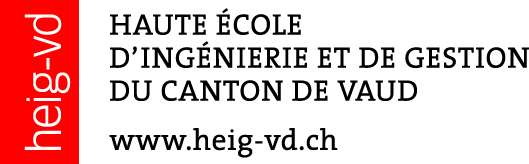
\includegraphics[scale=0.5]{HEIG-VD.png}}
\fancyhead[C]{}
%\fancyhead[R]{\small Travail de Bachelor - Pré-étude\\Bise Léonard\\Informatique Embarquée (ISEC)}
\fancyhead[R]{\small \leftmark}
%\fancyfoot{}

\begin{document}

\pagestyle{fancy}

\LARGE{Résumé}

\begin{normalsize}
Les compétitions sportives, de course à pied ou de cyclisme par exemple, sont des événements dont le déroulement n'est pas toujours facile à suivre pour les spectateurs qui sont sur place. Une fois le départ de la course donné, on peut vite perdre de vue les concurrents. Il faut donc se déplacer pour pouvoir suivre son déroulement et même dans ce cas, vu que le nombre de sportifs est souvent élevé, on peut difficilement se faire une idée globale sur la position de chacun d'eux ou du classement à un instant précis.

Ce projet propose la réalisation d’un système permettant le suivi en temps réel de compétitions sportives au travers d’une application mobile Android afin d'impliquer d'avantage les spectateurs. Grâce à une carte sur laquelle il est possible de voir le parcours de la course en entier, l'application tiendra à jour la position GPS de chaque coureur en temps réel au travers de données transmises par un capteur porté par les sportifs. L'interface propose également d'autres informations: le nom du sportif, son pays d'origine, son numéro de dossard, la distance parcourue, la vitesse moyenne, son rythme cardiaque et sa cadence (nombre de pas par unité de temps). Enfin, l'application permet de choisir ses coureurs favoris afin d'en faciliter le suivi ainsi que l'administration du système telles que la création des courses ou l'inscription des coureurs par exemple.

Pour que le système puisse remplir sa tâche, les éléments suivant ont été développés.

\begin{itemize}
\item Un capteur qui est porté par les athlètes et qui permet l'acquisition des données
\item Une passerelle qui est placée le long du parcours et qui centralise les données produites par les capteurs dans une base de données
\item Une application mobile qui permet la visualisation des données produites
\end{itemize}

La communication entre le capteur et la passerelle est assurée grâce à la technologie sans-fil LoRa, un protocole qui est prévu pour être utilisé par de petits systèmes avec peu de ressources sur des distances de plusieurs kilomètres, et qui ne nécessite pas de surcoût pour son utilisation contrairement aux communications mobiles GSM par exemple, car il utilise les bandes de fréquences libres ISM.

Le capteur dispose d'un micro-contrôleur ATSAMD21 avec un cœur ARM Cortex-M0+ sur lequel s'exécute le firmware développé pendant le travail de Bachelor. Il est écrit en C et utilise le système d'exploitation temps réel Zephyr qui propose tous les mécanismes et services nécessaires pour le développement d'une application embarquée temps réel.

La passerelle est construite à partir d'un Raspberry Pi 3 model B+ exécutant le système d'exploitation Linux ainsi que d'une carte de gestion de la couche radio LoRa. Une application serveur, codée en C++, se charge de récupérer les paquets reçus par l'interface LoRa et d'enregistrer les données décodées dans la base de données.

L'application mobile est développée en Java sur Android Studio et utilise le framework "Maps SDK for Android" de Google afin de gérer la carte et les éléments affichés dessus.

\end{normalsize}

\end{document}